%%%%%%%%%%%%%%%%%%%%%%%%%%%%%%%%%%%%%%%%%
% Szablon pracy dyplomowej
% Wydział Informatyki 
% Zachodniopomorski Uniwersytet Technologiczny w Szczecinie
% autor Joanna Kołodziejczyk (jkolodziejczyk@zut.edu.pl)
% Bardzo wczesnym pierwowzorem szablonu był
% The Legrand Orange Book
% Version 5.0 (29/05/2025)
%
% Modifications to LOB assigned by %JK
%%%%%%%%%%%%%%%%%%%%%%%%%%%%%%%%%%%%%%%%%


%----------------------------------------------------------------------------------------
%	CHAPTER 4
%----------------------------------------------------------------------------------------
\sloppy

\lstdefinestyle{csharp}{
	language=[Sharp]C,
	basicstyle=\ttfamily\small,
	keywordstyle=\color{blue},
	stringstyle=\color{red},
	commentstyle=\color{gray},
	numbers=left,
	numberstyle=\tiny,
	stepnumber=1,
	numbersep=5pt,
	frame=single,
	breaklines=true,
	captionpos=b,
	showtabs=false
}
\lstdefinelanguage{TypeScript}{
	language=Java,
	morekeywords={interface, type, implements, readonly, public, private, protected, enum, as, unknown, never},
	sensitive=true
}

\lstdefinestyle{tsstyle}{
	language=TypeScript,
	basicstyle=\ttfamily\small,
	keywordstyle=\color{blue},
	stringstyle=\color{red},
	commentstyle=\color{gray},
	numbers=left,
	numberstyle=\tiny,
	stepnumber=1,
	numbersep=5pt,
	frame=single,
	breaklines=true,
	tabsize=2,
	showtabs=false,
	showstringspaces=false
}

\chapter{Implementacja}
\label{rozdzial4}

\section{Środowisko i narzędzia programistyczne}
\index{Środowisko i narzędzia programistyczne}

\subsection{Zintegrowane środowisko programistyczne (IDE)}
\index{Zintegrowane środowisko programistyczne (IDE)}

Do pracy nad systemem wykorzystywane są narzędzia firmy JetBrains. Jetbrains IDE\footnote{Zintegrowane środowisko programistyczne, IDE – program lub zespół programów służących do tworzenia, modyfikowania, testowania i konserwacji oprogramowania.\cite{wikipedia.pl}} WebStorm dla prac Frontendowych Angular oraz IDE Rider do pracy z kodem C\# i Asp.Net Core. Są to zaawansowane narzędzia developerskie zapewniające kompleksowe wsparcie dla wybranych technologii.

\subsection{Narzędzia wspomagające rozwój oprogramowania}
\index{Narzędzia wspomagające rozwój oprogramowania}

Do śledzenia zmian kodu, wersjonowania oraz dla bezpieczeństwa projekt kod i wszystkie niezbędne pliki są przechowywane w systemie Git. Repozytorium Git\footnote{Git to rozproszony system kontroli wersji stworzony przez Linus'a Torvalds'a. Jest to aktualnie najczęściej wykorzystywane narzędzie do wersjonowania kodu na świecie, zarówno wśród hobbystów i pasjonatów programowania jak i w środowiskach profesjonalnych i biznesach.} znajduję się w serwisie Github\footnote{https://github.com/}.

\subsection{Środowisko uruchomieniowe i infrastruktura}
\index{Środowisko uruchomieniowe i infrastruktura}

\subsubsection{Maszyna deweloperska}
Konfiguracja maszyny deweloperskiej jest następująca:
\begin{itemize}
	\item \textbf{System operacyjny} - Windows 11
	\item \textbf{Serwer web} - Microsoft IIS oraz Node.js
	\item \textbf{Środowisko .NET} - .NET Core SDK 8.0.15
	\item \textbf{Środowisko Node.js} - Node v22 LTS
	\item \textbf{IDE} - JetBrains Rider 2024.3.* oraz JetBrains WebStorm 2024.3.6
\end{itemize}

\subsubsection{Serwer produkcyjny}
\begin{itemize}
	\item \textbf{System operacyjny} - Ubuntu 24.04 LTS
	\item \textbf{Serwer web} - Nginx oraz Node.js
	\item \textbf{Środowisko .NET} - .NET Core Runtime 8.0.15
	\item \textbf{Środowisko Node.js} - Node v22 LTS
\end{itemize}

\section{Struktura projektu}
\index{Struktura projektu}

Projekt został logicznie podzielony na dwie części. Pierwsza część frontendowa w technologii Angular z wykorzystaniem środowiska Node.js oraz npm. Drugą cześć to backend ASP.NET Core wraz z bazą danych SQLite3 wykorzystujące platformę .NET Core.

\subsection{Struktura folderów}
\index{Struktura folderów}

\subsubsection{Frontend}
Poniżej została przedstawiona struktura projektu Angular:
\begin{itemize}
	\item \textbf{public} - znajdują się w nim stałe grafiki strony
	\item \textbf{src} - katalog z kodem źródłowym aplikacji wraz z plikami index.html, main.ts oraz styles.scss
		\begin{itemize}
			\item \textbf{app} - kody źródłowe z podziałem na kolejne katalogi oraz głównym componentem applikacji i konfiguracją route
				\begin{itemize}
					\item \textbf{components} - komponenty składające się z kodu .ts oraz szablonu .html wykorzystywane wielokrotnie w aplikacji
					\item \textbf{interceptors}
					\item \textbf{models} - klasy wykorzystywane do przechowywania danych pobieranych z backendu
					\item \textbf{pages} - komponenty .ts i szablony .html tworzące strony, dialogi oraz formularze poszczególnych funkcjonalności serwisu
					\item \textbf{services} - serwisy wykorzystywane do autoryzacji i komunikacji z backendem
				\end{itemize}
			\item \textbf{environments} - pliki z danymi konfiguracyjnymi dla środowiska deweloperskiego i produkcyjnego
		\end{itemize}
\end{itemize}

\subsubsection{Backend}
Poniżej wylistowano strukturę projektu ASP.NET Core:
\begin{itemize}
	\item \textbf{Constants} - klasy ze stałymi wykorzystywane w projekcie
	\item \textbf{Controllers} - kontrolery REST API
	\item \textbf{Data} - kontekst bazodanowy oraz klasa obsługująca tworzenie nowej bazy z podstawową zawartością
	\item \textbf{Interfaces} - pliki interfejsów C\# implementowanych w aplikacji
	\item \textbf{Migrations} - migracje SQL tworzone przy modyfikacji modelów danych C\# i wykorzystywane do tworzenia i aktualizacji struktury bazy danych
	\item \textbf{Models} - modele danych w postaci klas C\# wykorzystywane w bazie danych oraz w komunikacji z Frontendem
		\begin{itemize}
			\item \textbf{DTOs} - uproszczone modele danych wykorzystywane w komunikacji z Frontendem
		\end{itemize}
	\item \textbf{Properties} - pliki konfiguracyjne uruchamiania
	\item \textbf{Services} - serwisy służące do autoryzacji i komunikacji z bazą danych
	\item \textbf{wwwroot} - folder zawierający przesyłane obrazy do aplikacji, dostępny z poziomu frontendu
\end{itemize}

\subsection{Technologie i zależności}
\index{Technologie i zależności}

\subsubsection{REST API}
W projekcie wymiana danych pomiędzy frontendem i backendem odbywa się za pomocą REST API, a dane są serializowane/deserializowane w standardzie JSON\footnote{JSON to skrót od JavaScript Object Notation (JavaScript Object Notation) JSON to lekki format do przechowywania i transportu danych. Z ang. \cite{w3s_json}}.

\begin{lstlisting}[style=tsstyle, caption=Przykład danych w formacie JSON]
{
"employees":[
	{"firstName":"John", "lastName":"Doe"},
	{"firstName":"Anna", "lastName":"Smith"},
	{"firstName":"Peter", "lastName":"Jones"}
]
}
\end{lstlisting}

\begin{lstlisting}[style=csharp, caption={Fragment kontrolera REST API z projektu}, label={lst:przykladCSController}]
namespace BackendService.Controllers
{
	[ApiController]
	[Route("api/[controller]")]
	public class BirdsController : ControllerBase
	{
		private readonly ApplicationDbContext _context;
		private readonly IBirdService _birdService;

		public BirdsController(ApplicationDbContext context, IBirdService birdService)
		{
			_context = context;
			_birdService = birdService;
		}

		[HttpGet]
		public async Task<ActionResult<PaginatedResponse<Bird>>> GetBirds([FromQuery] PaginationParams paginationParams)
		{
			var birds = await _birdService.GetAllBirdsAsync(paginationParams);
			return Ok(birds);
		}
...
\end{lstlisting}

\begin{lstlisting}[style=tsstyle, caption={Fragment serwisu po stronie frontendu}, label={lst:przykladTSService}]
@Injectable({
	providedIn: 'root'
})
export class BirdService {
	private baseUrl = `${environment.api.baseUrl}
		${environment.api.endpoints.birds}`;
	
	constructor(
	private http: HttpClient,
	private router: Router
	) { }
	
	private handleError(error: HttpErrorResponse) {
		if (error.status === 401 || error.status === 403) {
			// Przekieruj do strony logowania
			this.router.navigate(['/login'], { 
				queryParams: { 
					returnUrl: this.router.url 
				}
			});
		}
		return throwError(() => error);
	}
	
	getAllBirds(paginationParams: PaginationParams): Observable<PaginatedResponse<Bird>> {
		const params = new HttpParams()
		.set('pageNumber', paginationParams.pageNumber.toString())
		.set('pageSize', paginationParams.pageSize.toString());
		return this.http.get<PaginatedResponse<Bird>>(
			this.baseUrl, { params })
		.pipe(catchError(this.handleError.bind(this)));
	}
...
\end{lstlisting}

\subsubsection{ORM}
Do mapowania obiektowo-relacyjnego wykorzystywany jest Entity Framework Core. Umożliwia on pracę na platformie .NET z bazami danych przy użyciu kontekstu oraz modeli danych. Wykonywanie zapytań bazodanowych odbywa się w tle a programistą udostępniony jest wygodny interfejs LINQ\footnote{Zapytanie zintegrowane z językiem (LINQ) - zestaw technologii opartych na integracji funkcji zapytań bezpośrednio w języku C\#\cite{dotnet_linq}} niewymagający ręcznego pisania zapytań.

Przykład takiego wywołania zapytań został przedstawiony poniżej:
\begin{lstlisting}[style=csharp, caption={Przykład wywołania zapytania bazodanowego za pomocą EF Core oraz LINQ}]
var query = _context.Birds.Where(b =>
	b.IsVerified && (
	b.CommonName.ToLower().Contains(searchTerm) ||
	b.ScientificName.ToLower().Contains(searchTerm) ||
	b.Family.ToLower().Contains(searchTerm) ||
	b.Description.ToLower().Contains(searchTerm)
	)
);
\end{lstlisting}

\section{Implementacja frontendu}
\index{Implementacja frontendu}

\subsection{Zastosowane technologie}
W implementacji frontendu zostały wykorzystane poniżej wymienione technologie:
\begin{itemize}
	\item Angular 17 - framework
	\item Typescript, HTML5, CSS3 - języki programowania oraz znaczników i stylów
	\item Angular Material - biblioteka komponentów UI
	\item Leaflet - biblioteka do obsługi map interaktywnych
	\item RxJS - biblioteka do programowania reaktywnego
\end{itemize}

\subsection{Wzorce architektoniczne}
Aplikacja została wykonana w oparciu o obowiązujące trendy i odpowiednie wzorce architektoniczne wykorzystywane w programowaniu i zastosowaniu frameworku Angular.

\subsubsection{Modularna architektura}
Aplikacja jest podzielona na funkcjonalne moduły obsługujące poszczególne funkcjonalności takie jak zarządzanie stanem, logowaniem, wymianą danych z backendem oraz poszczególne komponenty stron i podstron.
Rozwój aplikacji w takiej konfiguracji jest efektywny - z łatwością można dodać kolejne elementy i wykorzystywać dependecy injection to zarządzania stanem i wykorzystania serwisów.

\subsubsection{Komponenty}
System składa się z komponentów Angular, które odpowiadają za poszczególne funkcjonalności i są reużywalne w całej aplikacji np.: pasek nawigacyjny, strony listującej ptaki, obserwacje, komponent formularzy, komponent obsługi mapy, logowania i rejestracji.
Każdy komponent składa się z pliku TypeScript zawierającego logikę biznesową danego komponentu oraz szablonu html ze stylami css do określenia wyglądu.

\begin{lstlisting}[style=tsstyle, caption={Fragment kodu TypeScript komponentu}]
@Component({
	selector: 'app-bird-details',
	standalone: true,
	imports: [ ... ],
	templateUrl: './bird-details.component.html',
	styleUrl: './bird-details.component.scss'
})
export default class BirdDetailsComponent implements OnInit {
	baseUrl = environment.api.baseUrl;
	bird: Bird | null = null;
	isLoading = true;
	errorMessage = '';
	isAdmin = false;
	dateFormat: string;
	
	constructor(
	private route: ActivatedRoute,
	private router: Router,
	private birdService: BirdService,
	private authService: AuthService,
	private snackBar: MatSnackBar,
	private dialog: MatDialog,
	private localeService: LocaleService,
	private userService: UserService
	) {
		this.dateFormat = this.localeService.getDateTimeFormat();
	}
	
	ngOnInit(): void {
		this.route.params.subscribe(params => {
			const id = params['id'];
			if (id) {
				this.loadBird(id);
			}
		});
		this.isAdmin = this.userService.isAdmin();
	}
	
	private loadBird(id: string): void {
		this.isLoading = true;
		this.birdService.getBirdById(Number(id)).subscribe({
			next: (bird) => {
				this.bird = bird;
				this.isLoading = false;
			},
			error: (error) => {
				this.errorMessage = 'Wystąpił błąd podczas ładowania danych ptaka';
				this.isLoading = false;
				console.error('Error loading bird:', error);
			}
		});
	}
...
\end{lstlisting}

\begin{lstlisting}[language=html, caption={Fragment szablonu html komponentu}]
<div class="container">
@if (isLoading) {
	<div class="loading-container">
	<mat-spinner></mat-spinner>
	</div>
} @else if (errorMessage) {
	<div class="error-message">
	{{ errorMessage }}
	</div>
} @else if (bird) {
	<mat-card class="bird-card">
	<div class="bird-content">
	<div class="bird-image">
	<img [src]="bird.imageUrl ? baseUrl + bird.imageUrl : baseUrl + '/images/placeholder.jpg'" [alt]="bird.commonName">
	</div>
	<div class="bird-info">
	<h1>{{ bird.commonName }}</h1>
	<h2>{{ bird.scientificName }}</h2>
...
\end{lstlisting}

\begin{lstlisting}[language=css, caption={Fragment styli css komponentu}]
.container {
	padding: 20px;
	max-width: 1200px;
	margin: 0 auto;
	min-height: 100vh;
	display: flex;
	flex-direction: column;
}

.loading-container {
	display: flex;
	justify-content: center;
	align-items: center;
	min-height: 400px;
}
...
\end{lstlisting}

\subsubsection{Serwisy}
Do komunikacji z backendem i implementacji logiki biznesowej wykorzystywane są serwisy. Serwisy są podzielone zgodnie z ich przeznaczeniem, np.: serwis do obsługi pobierania, dodawania, edycji ptaków, serwis autoryzacji użytkowników i uprawnień, serwis obserwacji.
Dodanie kolejnej funkcjonalności odbywa się przez dodanie kolejnego serwisu lub modyfikacji istniejącego i późniejszego wykorzystania go w komponentach. Fragment kody serwisu został przedstawiony w listingu \ref{lst:przykladTSService}.

\subsubsection{Routing}
Nawigacja między stronami została zrealizowana przy użyciu mechanizmów routingu wbudowanych w framework Angular.
\begin{lstlisting}[style=tsstyle, caption={Fragment kodu routingu}]
export const routes: Routes = [
{ path: '', component: HomePageComponent },
{
	path: 'birds',
	loadComponent: () => import('./pages/birds/birds.component').then(m => m.default)
},
{
	path: 'observations',
	loadComponent: () => import('./pages/observations/observations.component')
			.then(m => m.default)
},
{
	path: 'observations/add',
	loadComponent: () => import('./pages/add-observation/add-observation
			.component').then(m => m.default)
},
{
	path: 'observations/:id',
	loadComponent: () => import('./pages/observation-details/observation
			-details.component').then(m => m.default)
},
{
	path: 'observations/:id/edit',
	loadComponent: () => import('./pages/edit-observation/edit-observation
			.component').then(m => m.default)
},
...
\end{lstlisting}

\subsection{Implementacja komponentów głównych}

\subsubsection{Pasek nawigacyjny}
Pasek nawigacyjny jest stałym elementem na górze strony umożliwiającym nawigacje oraz logowanie i rejestracje. Responsywnie dostosowuje się do szerokości strony i na mniejszych ekranach przechodzi w tryb menu rozwijanego.

\begin{figure}[h]
	\centering
	
\includegraphics[width=1.0\textwidth]{/chapter4/navbar1.png}
	\caption{Pasek nawigacyjny na dużym ekranie}
	\label{fig:navbar1}
\end{figure}

\begin{figure}[h]
	\centering
	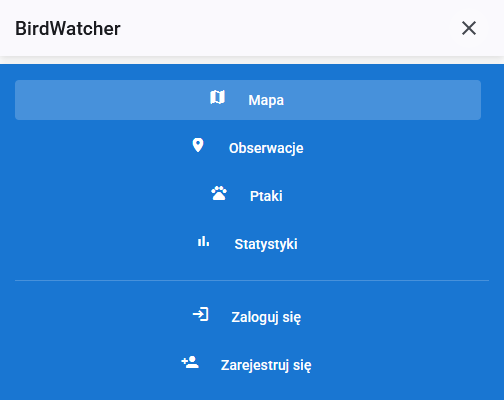
\includegraphics[width=0.6\textwidth]{/chapter4/navbar2.png}
	\caption{Pasek nawigacyjny w trybie rozwijanym}
	\label{fig:navbar2}
\end{figure}

\subsubsection{}

\section{Implementacja backendu}
\index{Implementacja backendu}

\section{Implementacja bazy danych}
\index{Implementacja bazy danych}

\section{Implementacja systemu autentyfikacji i autoryzacji}
\index{Implementacja systemu autentyfikacji i autoryzacji}

\section{Implementacja funkcjonalności mapy i geolokalizacji}
\index{Implementacja funkcjonalności mapy i geolokalizacji}